% Канонический TikZ-рисунок варианта 25. Править только здесь.
\long\def\figStereoV25{%
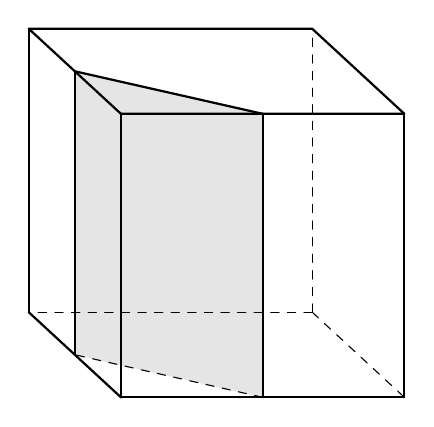
\begin{tikzpicture}[
  scale=0.9,
  line cap=round,
  line join=round
]
  % Вершины куба
  \coordinate (A)  at (0,0);
  \coordinate (B)  at (4,0);
  \coordinate (D)  at (-1.3,1.2);
  \coordinate (C)  at (2.7,1.2);

  \coordinate (A1) at (0,4);
  \coordinate (B1) at (4,4);
  \coordinate (D1) at (-1.3,5.2);
  \coordinate (C1) at (2.7,5.2);

  % Середины
  \coordinate (M)  at (2,0);
  \coordinate (N)  at (-0.65,0.6);
  \coordinate (M1) at (2,4);
  \coordinate (N1) at (-0.65,4.6);

  % Плоскость сечения
  \fill[black!10] (M)--(N)--(N1)--(M1)--cycle;

  % Куб
  \draw[thick] (A)--(B);
  \draw[dashed] (C)--(D);
  \draw[thick] (A)--(D);
  \draw[dashed] (C)--(B);
  \draw[thick] (A1)--(B1)--(C1)--(D1)--cycle;
  \draw[thick] (A)--(A1);
  \draw[thick] (B)--(B1);
  \draw[dashed] (C)--(C1);
  \draw[thick] (D)--(D1);

  % Отсекаемая треугольная призма

  \draw[thick] (A)--(A1);
  \draw[thick] (M)--(M1);
  \draw[thick] (N)--(N1);

  % След плоскости
  \draw[dashed] (M)--(N);
  \draw[thick] (M1)--(N1);
\end{tikzpicture}
}
